% =====================================================================
%  BreachShield: AI Powered OSINT Breach Detection & Dark Web Protection
%  Two-column conference-style layout (US Letter, Times, 10 pt)
%
%  HOW TO COMPILE
%    - Overleaf: upload this single file, set the compiler to pdfLaTeX, press Recompile.
%    - Local:    pdflatex BreachShield_Paper.tex   (run it twice so the references settle)
%
%  This file is fully self-contained. All figures are drawn inside the file
%  with TikZ / pgfplots, so no image files are needed. Only standard packages
%  are used (all ship with TeX Live and Overleaf).
% =====================================================================
\documentclass[10pt,twocolumn]{article}
\usepackage[letterpaper,top=0.75in,bottom=1in,left=0.625in,right=0.625in,columnsep=0.25in]{geometry}
\usepackage[T1]{fontenc}
\usepackage[utf8]{inputenc}
\usepackage{mathptmx}
\usepackage{microtype}
\usepackage{amsmath,amssymb}
\usepackage{tikz}
\usetikzlibrary{arrows.meta,positioning,calc}
\usepackage{pgfplots}
\pgfplotsset{compat=newest}
\usepackage{titlesec}
\usepackage{enumitem}
\usepackage{caption}
\usepackage{url}
\usepackage[hidelinks,pdftitle={BreachShield: AI Powered OSINT Breach Detection \& Dark Web Protection}]{hyperref}

\pagestyle{empty}
\setlength{\parindent}{1.0em}
\setlength{\parskip}{0pt}
\linespread{0.98}
\tolerance=1000
\emergencystretch=1em
\urlstyle{same}
\widowpenalty=10000
\clubpenalty=10000

% ---------- IEEE-style headings ----------
\renewcommand{\thesection}{\Roman{section}}
\renewcommand{\thesubsection}{\Alph{subsection}}
\titleformat{\section}[block]{\centering\normalfont\normalsize\scshape}{\thesection.}{0.6em}{}
\titlespacing*{\section}{0pt}{9pt}{4pt}
\titleformat{\subsection}[block]{\normalfont\normalsize\itshape}{\thesubsection.}{0.5em}{}
\titlespacing*{\subsection}{0pt}{6pt}{2pt}

% ---------- captions and lists ----------
\captionsetup[figure]{name={Fig.},labelsep=period,font=footnotesize,justification=justified,singlelinecheck=true,skip=3pt}
\setlist{nosep,leftmargin=1.4em,itemsep=1pt,topsep=2pt}

% ---------- table helpers ----------
\newcommand{\tcap}[2]{\begin{center}\footnotesize TABLE #1\\[1pt]\scshape #2\end{center}\vspace{-8pt}}
\newcommand{\tnote}[1]{\par\vspace{2pt}{\footnotesize #1\par}}

% ---------- algorithm helpers ----------
\newcommand{\algtop}[1]{\noindent\rule{\columnwidth}{0.6pt}\\[1pt]{\footnotesize\textbf{#1}}\\[-1pt]\rule{\columnwidth}{0.4pt}}
\newcommand{\algmid}{\noindent\rule{\columnwidth}{0.4pt}}
\newcommand{\algbot}{\noindent\rule{\columnwidth}{0.6pt}}
\newcommand{\cmt}[1]{\hfill$\triangleright$\,\textit{#1}}
\newcommand{\algtab}[1]{\par\vspace{1pt}\noindent\begin{tabular}{@{}r@{\hspace{5pt}}p{0.9\columnwidth}@{}}#1\end{tabular}\par}

% ---------- plot colours ----------
\definecolor{bsblue}{RGB}{31,95,168}
\definecolor{bsgray}{RGB}{127,140,141}
\definecolor{bsgold}{RGB}{217,164,65}
\definecolor{bsred}{RGB}{192,57,43}

\begin{document}

% =====================  TITLE BLOCK  =====================
\twocolumn[{%
\centering
{\fontsize{22}{25}\selectfont BreachShield: AI Powered OSINT Breach Detection \& Dark Web Protection\par}
\vspace{10pt}
\footnotesize
\begin{minipage}[t]{0.32\textwidth}\centering
\textbf{Sushma T. M. (Project Guide)}\\
\textit{Assistant Professor}\\
\textit{Dept. of Information Science \& Engineering}\\
\textit{Acharya Institute of Technology}\\
Bengaluru, India\\
sushma2471@acharya.ac.in
\end{minipage}\hfill
\begin{minipage}[t]{0.32\textwidth}\centering
\textbf{Arvind D. H}\\
\textit{Dept. of Information Science \& Engineering}\\
\textit{Acharya Institute of Technology}\\
Bengaluru, India\\
arvindd.24.beis@acharya.ac.in
\end{minipage}\hfill
\begin{minipage}[t]{0.32\textwidth}\centering
\textbf{Girishkumar N. M}\\
\textit{Dept. of Information Science \& Engineering}\\
\textit{Acharya Institute of Technology}\\
Bengaluru, India\\
girishkumarn.24.beis@acharya.ac.in
\end{minipage}

\vspace{8pt}
\hfill
\begin{minipage}[t]{0.32\textwidth}\centering
\textbf{Manoj}\\
\textit{Dept. of Information Science \& Engineering}\\
\textit{Acharya Institute of Technology}\\
Bengaluru, India\\
manojl.24.beis@acharya.ac.in
\end{minipage}\hspace{0.04\textwidth}%
\begin{minipage}[t]{0.32\textwidth}\centering
\textbf{Premkumar Teli}\\
\textit{Dept. of Information Science \& Engineering}\\
\textit{Acharya Institute of Technology}\\
Bengaluru, India\\
premkumard.24.beis@acharya.ac.in
\end{minipage}
\hfill\mbox{}
\vspace{12pt}
}]

% =====================  ABSTRACT  =====================
\noindent\textbf{\textit{Abstract}---\,Breach lookup services have a privacy problem built into their design. To find out whether an e-mail address or phone number has leaked, people usually have to hand that same identifier to a third-party server, which turns a protective tool into a possible point of surveillance. BreachShield is an open-source-intelligence platform that keeps plaintext identifiers out of the lookup path. The browser hashes the identifier with SHA-256 and sends only a 20-bit prefix of the digest. Around this query we built an out-of-band one-time-password gate, a deterministic and explainable exposure score, a pluggable registry of breach sources, and a Merkle-batched audit log designed to be anchored on an Ethereum Virtual Machine (EVM) smart contract. We analyse what each channel reveals. The anonymity set grows linearly with the size of the indexed corpus, so at our current corpus size the guarantee is weak, and we say so openly. We also show that the authentication channel can expose the queried identifier to the operator. On 1,034 curated breach records, a gradient-boosted tree classifier reaches 89.2\% test accuracy (95\% confidence interval 83.3--93.1) and 83.2\% macro F1, compared with 66.2\% and 57.2\% for the strongest neural baseline. The back-end and front-end test suites pass in full (101 of 101 and 50 of 50). We re-checked every reported result by running the system or reading its source, and anything we could not verify, including end-to-end blockchain anchoring, is reported as a limitation rather than as a result.}

\vspace{6pt}
\noindent\textbf{\textit{Keywords}---\,breach intelligence, k-anonymity, OSINT, Merkle tree, tamper-evident logging, XGBoost, privacy-preserving search}

% =====================  I. INTRODUCTION  =====================
\section{Introduction}

In IBM's 2024 study, compromised credentials were the most common initial attack vector, accounting for 16\% of the breaches examined, and the global average cost of a breach reached USD 4.88 million [1]. A service that tells people whether their details appear in a breach corpus is therefore clearly useful, and breach alerting at scale has been studied as a way to protect accounts from credential stuffing [2]. The lookup itself, however, is a privacy risk. A service that asks for a plaintext e-mail address or phone number in order to report its exposure can store, correlate or leak the very identifiers it is supposed to protect.

The k-anonymity range query solves part of this problem. The client hashes the secret, discloses only a short prefix of the hash, receives every corpus entry that shares that prefix, and finishes the comparison locally. The construction was deployed for Pwned Passwords [3] and has been analysed, along with stronger private-set-intersection alternatives, by Li \textit{et al.} [4]. Three questions remain open once the technique is placed inside a multi-tenant breach-intelligence platform. First, requests are usually authenticated so that usage can be held accountable, and an authenticated channel carries information that the hash prefix does not. Second, the size of the anonymity set is set by the indexed corpus, and a domain-specific or academic platform has only a small one. Third, a platform that accepts lookups needs an audit trail whose integrity does not depend on trusting the operator, yet writing one blockchain transaction per query is impractical.

We study these questions through BreachShield, an open-source-intelligence (OSINT) breach platform made up of a React client, an Express gateway, a Python OSINT microservice, an Android SMS relay and a smart-contract anchor. We ask three research questions. \textbf{RQ1}: what does a prefix-range lookup disclose when it is gated by an authenticated session, and how large is the resulting anonymity set? \textbf{RQ2}: how can lookups be logged in a tamper-evident way at a bounded on-chain cost, and what exposure window does batching leave? \textbf{RQ3}: how do tree-based and neural classifiers compare for breach-severity triage on a small tabular dataset? Our contributions are as follows.
\begin{itemize}
\item A threat model and a per-channel leakage analysis of an authenticated k-anonymous range lookup, including a corpus-size analysis of the anonymity set that reproduces the bucket statistic reported for Pwned Passwords [3] (Section V).
\item A count-or-time Merkle batching scheme for audit events, anchored to an EVM smart contract, together with an analysis of the exposure window it leaves (Sections IV-E and V-C).
\item A deterministic, bounded and explainable exposure-scoring function (Algorithm 3).
\item A comparison of XGBoost with three neural baselines on 1,034 curated breach records, with confidence intervals computed from the reported test counts (Section VI).
\item A verification record, built by running or reading every component, that separates the behaviour we confirmed from the defects that remain open (Section VII).
\end{itemize}

% =====================  II. RELATED WORK  =====================
\section{Related Work}

\subsection{Compromised-Credential Checking and k-Anonymity}

Sweeney's k-anonymity model [5] and its application to health data [6] give the general guarantee that an individual cannot be distinguished from at least $k{-}1$ others in a released group.

Range queries bring this idea to lookups: the client reveals only a short prefix of a hash and filters the returned bucket on its own side. The Pwned Passwords service uses the first five hexadecimal characters of a SHA-1 hash and reports buckets of a few hundred entries over a corpus of hundreds of millions of hashes [3]. Li \textit{et al.} [4] analyse the security of compromised-credential-checking protocols of this kind and propose protocols with stronger guarantees based on private set intersection, at a higher protocol cost. BreachShield applies the range construction to hashed identifiers behind an authenticated gate, and Section V-A examines what that gate adds.

\subsection{Classification in Security Settings}

Deep models are widely used for phishing-URL detection. Aljofey \textit{et al.} [7] classify raw URL strings with a character-level CNN. Sahingoz \textit{et al.} [8] compare five deep architectures (ANN, CNN, RNN, bidirectional RNN and attention networks) on roughly five million labelled URLs and report that CNNs perform best, at 98.74\% accuracy. Alsubaei \textit{et al.} [9] find that SMOTE oversampling raises the accuracy of a hybrid deep phishing classifier from 83\% to 98\%, which is relevant to the scarce CRITICAL class in our data. Explainability [10] and few-shot learning [11] are active directions in phishing detection. All of these studies work with URL or text inputs. BreachShield uses a pretrained URL transformer for the URL signal and evaluates its classifiers separately on tabular breach metadata (Section VI).

\subsection{OSINT and Dark-Web Intelligence}

K\"uhn \textit{et al.} [12] evaluate manual and semi-automated use of the dark web for cyber threat intelligence. Saleem \textit{et al.} [13] survey the anonymity mechanisms behind dark-web infrastructure, and Pastor-Galindo \textit{et al.} [14] review the opportunities and open challenges of OSINT. BreachShield's source registry, whose adapters include a live Telegram-channel scraper, follows this direction on a small scale.

\subsection{Tamper-Evident Logging}

Merkle's hash trees [15] and the history trees of Crosby and Wallach [16] underlie append-only logs with efficient inclusion and consistency proofs, and Certificate Transparency [17] is a widely deployed log of this kind. Arabnouri \textit{et al.} [18] reduce on-chain storage by grouping log records into time-interval batches and recording only a checkpoint on the blockchain, with each record protected by a message authentication code. BreachShield shares the batching goal, but it flushes on record count as well as on time, and it anchors Merkle roots rather than checkpoints of chained MACs.

\subsection{Tabular Learning}

XGBoost [19] is a scalable gradient-boosted tree system. Grinsztajn \textit{et al.} [20] show that tree-based models still outperform deep networks on medium-sized tabular data, and they attribute the gap to the bias of neural networks toward smooth functions and to their sensitivity to uninformative features. Table I sets BreachShield's design choices beside the closest approaches discussed above.

\begin{table}[!t]
\centering
\tcap{I}{Design Comparison with Related Approaches}
\footnotesize
\setlength{\tabcolsep}{3pt}
\begin{tabular}{|p{0.18\columnwidth}|p{0.33\columnwidth}|p{0.40\columnwidth}|}
\hline
\textbf{Dimension} & \textbf{Related approach} & \textbf{BreachShield}\\
\hline
Query privacy & Hash-prefix k-anonymity for passwords [3], [4] & Same construction on hashed identifiers, with an authenticated gate added (Sec. V-A)\\
\hline
Audit anchoring & Time-interval checkpoints on a blockchain [18] & Count-or-time Merkle batches; local EVM node\\
\hline
Severity model & Deep models for URL text [8] & Tree ensemble on tabular metadata [20]\\
\hline
Class imbalance & SMOTE resampling [9] & Not yet applied (Sec. VIII)\\
\hline
\end{tabular}
\end{table}

% =====================  III. THREAT MODEL  =====================
\section{Threat Model and Requirements}

\textit{Setting.} A user wants to know whether an identifier $T$ (an e-mail address or a phone number) appears in a breach corpus held by the platform, without disclosing $T$. Three parties take part: the client, the gateway with its record store and source adapters, and the audit log with its on-chain anchor.

\textit{Adversaries.} We consider four adversaries: (A1) a network eavesdropper who observes client--gateway traffic; (A2) an honest-but-curious operator who follows the protocol faithfully but may inspect and retain everything the gateway receives, including authentication records; (A3) a malicious client that issues many queries to harvest buckets; and (A4) an insider who alters stored audit records after the fact. We do not consider a server that deviates from the protocol by returning fabricated buckets, or a client that tries to learn another user's exposure beyond what the authentication gate already prevents.

\textit{Requirements.} R1: no plaintext identifier or full hash appears on the range-query path. R2: the lookup request discloses only bounded information about the target digest to A2. R3: any change to an anchored audit event is detectable. R4: every lookup can be attributed to a verified identity. R5: a failing source or an unreachable microservice must not make the search fail.

% =====================  IV. SYSTEM DESIGN  =====================
\section{System Design}

\subsection{Architecture}

BreachShield is a four-tier monorepo (Fig.~\ref{fig:arch}). The React 19 client computes SHA-256 with the W3C Web Crypto API, so the search target is hashed in the browser before anything is sent. The Express 5 gateway issues and verifies one-time passwords, manages JWT sessions [21], dispatches each lookup to a pluggable breach-source registry, computes the exposure score and queues audit events. State is kept in MySQL 8, with an automatic fall-back to a JSON file. A FastAPI microservice hosts a Telethon-based Telegram scraper and a pretrained URL-transformer classifier (UrlBERT). Early on, concurrent requests that shared the scraper's session file caused database-locked errors, which we fixed by serialising access with an asyncio lock and an 8-second timeout. An Android application written in Kotlin keeps a WebSocket connection to the gateway and relays OTP codes as SMS, using templates that satisfy Indian DLT requirements. Carriers silently drop non-conforming payloads, so a fixed template format was required. Audit roots are anchored on a Hardhat EVM node.

\begin{figure}[!t]
\centering
\resizebox{\columnwidth}{!}{%
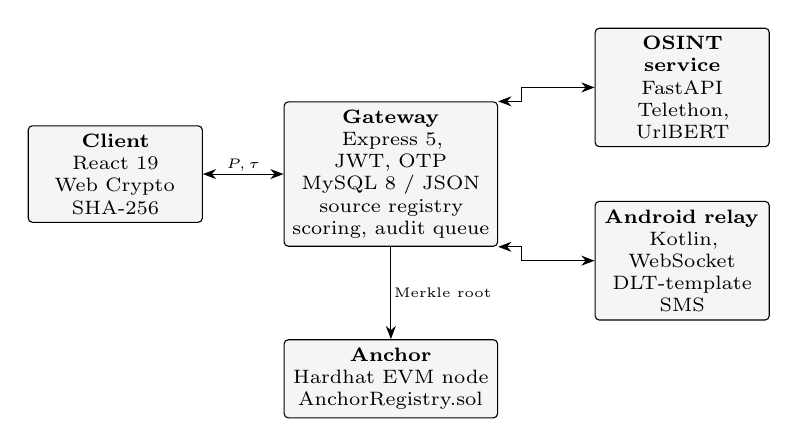
\begin{tikzpicture}[font=\scriptsize,>=Stealth,
  box/.style={draw,rounded corners=1.5pt,align=center,inner sep=3pt,fill=gray!8},
  lbl/.style={font=\tiny,inner sep=1pt}]
\node[box,text width=2.0cm] (cl) at (0,1) {\textbf{Client}\\React 19\\Web Crypto SHA-256};
\node[box,text width=2.5cm] (gw) at (3.5,1) {\textbf{Gateway}\\Express 5, JWT, OTP\\MySQL 8 / JSON\\source registry\\scoring, audit queue};
\node[box,text width=2.0cm] (os) at (7.2,2.1) {\textbf{OSINT service}\\FastAPI\\Telethon, UrlBERT};
\node[box,text width=2.0cm] (an) at (7.2,-0.1) {\textbf{Android relay}\\Kotlin, WebSocket\\DLT-template SMS};
\node[box,text width=2.5cm] (ch) at (3.5,-1.6) {\textbf{Anchor}\\Hardhat EVM node\\AnchorRegistry.sol};
\draw[<->] (cl.east) -- node[lbl,above]{$P,\tau$} (gw.west);
\draw[<->] (gw.north east) -- ++(0.3,0) |- (os.west);
\draw[<->] (gw.south east) -- ++(0.3,0) |- (an.west);
\draw[->] (gw.south) -- node[lbl,right]{Merkle root} (ch.north);
\end{tikzpicture}}
\caption{The four tiers of BreachShield and the data paths we confirmed between them.}
\label{fig:arch}
\end{figure}

The source registry defines an abstract BreachSource with a single \texttt{search(normalizedTarget, targetHash)} contract and four adapters. Two of them query real data: a local breach catalog and a live Telegram channel. The other two are registered placeholders that make no outbound calls. Lookups are dispatched concurrently with \texttt{Promise.allSettled}, so a failing source degrades the result instead of failing the request (R5).

\subsection{k-Anonymous Range Query}

The client normalises the identifier and computes the 256-bit digest $D$ as in \eqref{eq:hash}. It then splits $D$ into a 20-bit prefix $P$, which is five hexadecimal characters, and a 236-bit suffix $S$, as in \eqref{eq:split}. Only $P$ leaves the browser. The gateway returns the bucket $B(P)$, which contains every stored entry $(S_i, M_i)$ whose digest begins with $P$, and the client keeps the metadata $M_i$ of the entries whose suffix equals $S$ (Algorithm 1, Fig.~\ref{fig:seq}). The suffix comparison therefore never leaves the browser.
\begin{equation}
D=\mathrm{SHA\text{-}256}(T'),\qquad T'=\mathrm{lower}(\mathrm{trim}(T))
\label{eq:hash}
\end{equation}
\begin{equation}
D=P\,\|\,S,\qquad |P|=20\ \text{bits},\quad |S|=236\ \text{bits}
\label{eq:split}
\end{equation}

\begin{figure}[!t]
\algtop{Algorithm 1: Client-side k-anonymous range query}
\par\vspace{1pt}\noindent{\footnotesize\textbf{Input:} identifier $T$; session token $\tau$\\
\textbf{Output:} matched breach metadata $R$\par}
\algmid
{\footnotesize
\algtab{
1 & $T' \leftarrow \mathrm{lower}(\mathrm{trim}(T))$\\
2 & $D \leftarrow \mathrm{SHA\text{-}256}(T')$ \cmt{in the browser}\\
3 & $P \leftarrow$ first 5 hex characters of $D$; $S \leftarrow$ the remaining 59\\
4 & $B \leftarrow \mathrm{RangeQuery}(P,\tau)$ \cmt{only $P$ and $\tau$ are sent}\\
5 & $R \leftarrow \emptyset$\\
6 & \textbf{for each} $(S_i,M_i)\in B$ \textbf{do}\\
7 & \hspace{1em}\textbf{if} $S_i = S$ \textbf{then} $R \leftarrow R\cup\{M_i\}$\\
8 & \textbf{return} $R$}}
\algbot
\end{figure}

\begin{figure}[!t]
\centering
\resizebox{\columnwidth}{!}{%
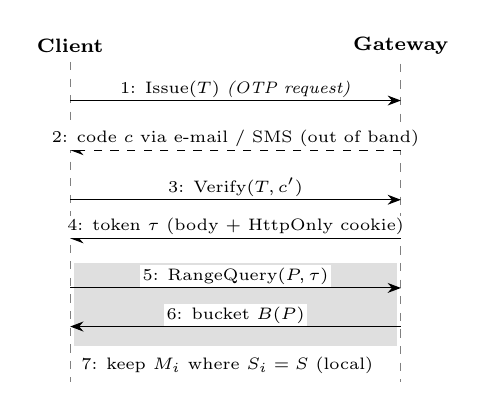
\begin{tikzpicture}[yscale=0.7,font=\scriptsize,>=Stealth,
  msg/.style={font=\fontsize{6}{7}\selectfont,inner sep=1pt,fill=white}]
\node (c) at (0,0) {\textbf{Client}};
\node (g) at (4.2,0) {\textbf{Gateway}};
\draw[dashed,gray] (c.south) -- (0,-6.1);
\draw[dashed,gray] (g.south) -- (4.2,-6.1);
\fill[gray!25] (0.05,-3.95) rectangle (4.15,-5.45);
\draw[->] (0,-1.0) -- node[msg,above]{1: Issue$(T)$ \textit{(OTP request)}} (4.2,-1.0);
\draw[->,dashed] (4.2,-1.9) -- node[msg,above]{2: code $c$ via e-mail / SMS (out of band)} (0,-1.9);
\draw[->] (0,-2.8) -- node[msg,above]{3: Verify$(T,c')$} (4.2,-2.8);
\draw[->] (4.2,-3.5) -- node[msg,above]{4: token $\tau$ (body + HttpOnly cookie)} (0,-3.5);
\draw[->] (0,-4.4) -- node[msg,above]{5: RangeQuery$(P,\tau)$} (4.2,-4.4);
\draw[->] (4.2,-5.1) -- node[msg,above]{6: bucket $B(P)$} (0,-5.1);
\node[msg,anchor=west] at (0.1,-5.8) {7: keep $M_i$ where $S_i=S$ (local)};
\end{tikzpicture}}
\caption{Range-query message sequence. The gateway observes only the prefix $P$ and the session token $\tau$ (shaded).}
\label{fig:seq}
\end{figure}

\subsection{Identity Gate}

Lookups are gated behind an OTP-verified session. The gate limits automated bucket harvesting (A3) and makes queries attributable (R4); Algorithm 2 gives the flow. A six-digit code from a cryptographically secure generator is hashed with bcrypt [22] at cost factor 10 and stored with a five-minute expiry. Resends are limited by a 30-second cooldown, and verification by a limit of five attempts. On success, the gateway issues a one-hour JWT whose claims carry the target identifier and a verified flag. The token is returned both in the response body and as an HttpOnly cookie, so later requests present the session rather than the code. Delivery is by e-mail or, for phone targets, by a DLT-templated SMS relayed through the Android gateway, and code records are kept in MySQL with an automatic JSON-file fallback if the database fails. Only the bcrypt hash of the code is persisted, so an operator who reads the OTP store learns the destination address but not the code.

\begin{figure}[!t]
\algtop{Algorithm 2: OTP issuance and verification}
\par\vspace{1pt}\noindent{\footnotesize\textbf{Input:} identifier $T$ (e-mail or phone); submitted code $c'$\\
\textbf{Output:} session token $\tau$, or rejection\par}
\algmid
{\footnotesize
\algtab{
1 & \textbf{Issue}$(T)$:\\
2 & \hspace{1em}\textbf{if} last send to $T$ was $<30$\,s ago \textbf{then reject}\\
3 & \hspace{1em}$c \leftarrow$ six-digit integer from a CSPRNG\\
4 & \hspace{1em}store (bcrypt$(c)$, expiry $=$ now $+$ 5 min, attempts $=0$)\\
5 & \hspace{1em}deliver $c$ by e-mail, or by DLT-templated SMS through the Android gateway\\
6 & \textbf{Verify}$(T,c')$:\\
7 & \hspace{1em}\textbf{if} expired \textbf{or} attempts $\ge 5$ \textbf{then reject}\\
8 & \hspace{1em}attempts $\leftarrow$ attempts $+1$\\
9 & \hspace{1em}\textbf{if} bcrypt-check$(c',$ stored hash$)$ \textbf{then}\\
10 & \hspace{2em}$\tau \leftarrow \mathrm{JWT}(T,\ \mathrm{verified}=\text{true},\ \mathrm{exp}=\text{now}+1\,\text{h})$\\
11 & \hspace{2em}\textbf{return} $\tau$ \cmt{response body and HttpOnly cookie}\\
12 & \hspace{1em}\textbf{else reject}}}
\algbot
\end{figure}

\subsection{Exposure-Risk Scoring}

The production scorer is a deterministic function of the aggregated multi-source result text, not of isolated structured fields. Regular expressions detect password and hash material, phone numbers, e-mail addresses, national-ID and document numbers, physical addresses and named relations. Points accumulate per category up to a cap (Table II). A cross-record correlation term adds up to 15 points and, when the URL classifier returns a phishing probability $p$, a further $30p$ points are added. The score is clamped to $[20,100]$ as in \eqref{eq:score} and mapped to one of four tiers: LOW, MEDIUM, HIGH or CRITICAL. Source reliability and breach recency are also derived from the aggregated text instead of being read from fixed constants. Because every contribution is a named, capped term, the result is returned together with its contributing factors.
\begin{equation}
s=\operatorname{clamp}\!\Big(\sum_{c}\min(\pi_c,\kappa_c)+\min(\rho,15)+30p,\ 20,\ 100\Big)
\label{eq:score}
\end{equation}

\begin{table}[!t]
\centering
\tcap{II}{Exposure-Score Components}
\footnotesize
\begin{tabular}{|l|c|}
\hline
\textbf{Component} & \textbf{Max. points}\\
\hline
Document or national-ID exposure & 35\\
\hline
Password or hash material & 30\\
\hline
Physical address & 20\\
\hline
Phone number & 15\\
\hline
Multiple independent sources & 15\\
\hline
Cross-record correlation ($\rho$) & 15\\
\hline
Phishing probability ($30p$) & 30\\
\hline
\end{tabular}
\tnote{The caps sum to 160, and the score is clamped to $[20,100]$. Here $\pi_c$ is the number of points earned in category $c$ and $\kappa_c$ is its cap.}
\end{table}

\begin{figure}[!t]
\algtop{Algorithm 3: Exposure-risk scoring}
\par\vspace{1pt}\noindent{\footnotesize\textbf{Input:} aggregated result text $X$; phishing probability $p$ (optional)\\
\textbf{Output:} score $s\in[20,100]$; tier; factors\par}
\algmid
{\footnotesize
\algtab{
1 & $s \leftarrow 0$\\
2 & \textbf{for each} category $c\in\{$document, password/hash, address, phone, multi-source$\}$ \textbf{do}\\
3 & \hspace{1em}$s \leftarrow s + \min(\pi_c(X),\kappa_c)$\\
4 & $s \leftarrow s + \min(\rho(X),15)$ \cmt{cross-record correlation}\\
5 & \textbf{if} $p$ is available \textbf{then} $s \leftarrow s + 30p$\\
6 & $s \leftarrow \operatorname{clamp}(s,20,100)$\\
7 & \textbf{return} $(s,\ \mathrm{tier}(s),\ \text{factors})$}}
\algbot
\end{figure}

\subsection{Audit Anchoring}

Each audit event is canonicalised as sorted-key JSON and hashed to a leaf. Leaves are queued and flushed into a Merkle tree when the queue reaches $B_{\max}$ entries or $T_{\max}=60$\,s have elapsed, whichever comes first (Algorithm 4, Fig.~\ref{fig:merkle}). The root is submitted to \texttt{AnchorRegistry.sol} with a batch identifier and the leaf count, and the gateway waits for the transaction receipt. Only the root is stored on-chain, so the chain provides integrity but not confidentiality of the event content.

\begin{figure}[!t]
\algtop{Algorithm 4: Merkle batching and on-chain anchoring}
\par\vspace{1pt}\noindent{\footnotesize\textbf{Input:} audit-event stream; thresholds $B_{\max}$, $T_{\max}$\\
\textbf{Output:} Merkle roots stored in AnchorRegistry\par}
\algmid
{\footnotesize
\algtab{
1 & $Q \leftarrow$ empty queue; $t_0 \leftarrow$ now\\
2 & \textbf{on} event $e$:\\
3 & \hspace{1em}$\ell \leftarrow \mathrm{SHA\text{-}256}(\mathrm{canon}(e))$ \cmt{sorted-key JSON}\\
4 & \hspace{1em}append $\ell$ to $Q$\\
5 & \hspace{1em}\textbf{if} $|Q|\ge B_{\max}$ \textbf{or} now $-\,t_0\ge T_{\max}$ \textbf{then} Flush()\\
6 & \textbf{Flush}() \cmt{also run when the timer expires}\\
7 & \hspace{1em}$R \leftarrow \mathrm{MerkleRoot}(Q)$\\
8 & \hspace{1em}submit anchorRoot(batchId, $R$, $|Q|$); await receipt\\
9 & \hspace{1em}$Q \leftarrow$ empty queue; $t_0 \leftarrow$ now}}
\algbot
\end{figure}

\begin{figure}[!t]
\centering
\resizebox{0.95\columnwidth}{!}{%
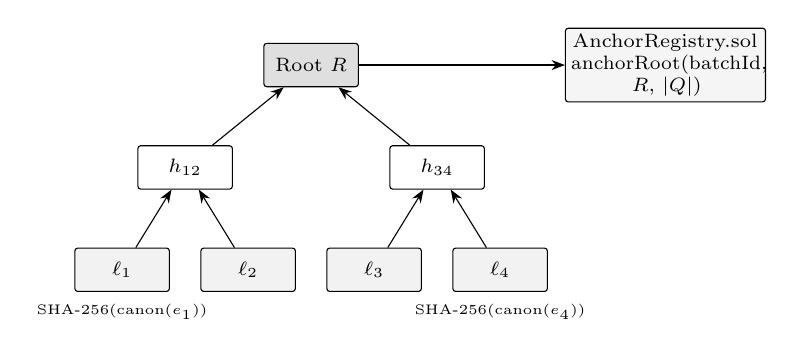
\begin{tikzpicture}[font=\scriptsize,>=Stealth,
  n/.style={draw,rounded corners=1pt,minimum width=1.2cm,minimum height=0.55cm,align=center,inner sep=2pt},
  lf/.style={n,fill=gray!10}]
\node[lf] (l1) at (0,0)   {$\ell_1$};
\node[lf] (l2) at (1.6,0) {$\ell_2$};
\node[lf] (l3) at (3.2,0) {$\ell_3$};
\node[lf] (l4) at (4.8,0) {$\ell_4$};
\node[n] (h12) at (0.8,1.3) {$h_{12}$};
\node[n] (h34) at (4.0,1.3) {$h_{34}$};
\node[n,fill=gray!25] (r) at (2.4,2.6) {Root $R$};
\draw[->] (l1) -- (h12); \draw[->] (l2) -- (h12);
\draw[->] (l3) -- (h34); \draw[->] (l4) -- (h34);
\draw[->] (h12) -- (r);  \draw[->] (h34) -- (r);
\node[font=\tiny,below=1pt of l1,align=center] {SHA-256(canon($e_1$))};
\node[font=\tiny,below=1pt of l4,align=center] {SHA-256(canon($e_4$))};
\node[n,text width=2.4cm,fill=gray!8] (ch) at (6.9,2.6) {AnchorRegistry.sol\\anchorRoot(batchId, $R$, $|Q|$)};
\draw[->] (r) -- (ch);
\end{tikzpicture}}
\caption{Merkle batching of audit events (illustrative four-leaf batch) and anchoring of the root $R$.}
\label{fig:merkle}
\end{figure}

% =====================  V. PRIVACY AND INTEGRITY  =====================
\section{Privacy and Integrity Analysis}

\subsection{What Each Channel Discloses}

The range request reveals a function of the target digest that takes at most $2^{20}$ values, so by the data-processing bound its leakage satisfies \eqref{eq:leak}. This bound concerns the request payload and does not depend on the corpus size.
\begin{equation}
I(D;P)\ \le\ H(P)\ \le\ \log_2 2^{20}=20\ \text{bits}
\label{eq:leak}
\end{equation}

The bound does not cover the other channels. The OTP step discloses the destination address or number to the gateway and to the e-mail or SMS path, and the session token carries the target identifier (Section IV-C). The authentication channel therefore discloses the full identifier to an operator who reads authentication records (A2), whatever the prefix protocol does, whenever the authenticated identifier is the one being searched. The range query still protects against the eavesdropper (A1) and against inference from query payloads, but not against an operator who joins those payloads with authentication logs. Accountability (R4) and privacy (R2) are therefore in tension, and we state the guarantee channel by channel instead of as an unconditional property. Two mitigations exist but are not implemented: authenticating with an account identifier that differs from the queried identifier, or replacing the prefix protocol with a private-set-intersection protocol [4].

\subsection{Anonymity-Set Size}

For a corpus of $N$ entries with uniformly distributed digests, the expected bucket size at a prefix length of $b$ bits is given by \eqref{eq:bucket}. With $b=20$ and $N=1{,}034$ the expectation is $9.9\times10^{-4}$, so a returned bucket is almost always empty or holds only the record being looked up. One expected record per bucket requires $N\ge 2^{20}\approx 1.05\times10^{6}$, and hundreds of records per bucket require hundreds of millions. As a check, \eqref{eq:bucket} predicts 305 entries per bucket for the 320-million-hash Pwned Passwords corpus, which agrees with the median bucket size of 305 reported for that corpus [3]. Fig.~\ref{fig:bucket} shows the dependence for three prefix lengths. Shorter prefixes enlarge the bucket and disclose fewer bits, but they transfer proportionally more data per query. At its present corpus size, BreachShield's privacy therefore rests on the 20-bit bound \eqref{eq:leak} rather than on a large anonymity set, and its k-anonymity property should be read as conditional on corpus growth.
\begin{equation}
E[k]=\frac{N}{2^{b}}
\label{eq:bucket}
\end{equation}

\begin{figure}[!t]
\centering
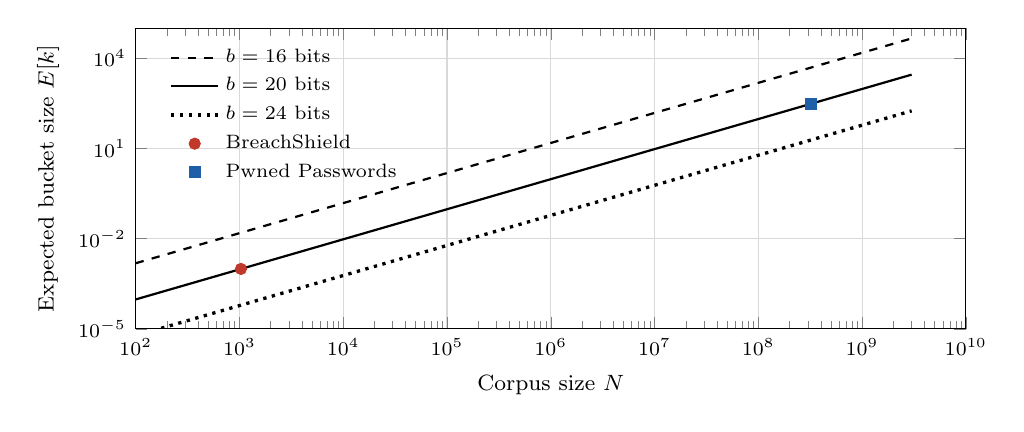
\begin{tikzpicture}
\begin{loglogaxis}[width=\columnwidth,height=5.4cm,
  xlabel={Corpus size $N$},ylabel={Expected bucket size $E[k]$},
  xmin=1e2,xmax=1e10,ymin=1e-5,ymax=1e5,
  grid=major,grid style={gray!30,thin},
  tick label style={font=\scriptsize},label style={font=\footnotesize},
  legend style={font=\scriptsize,draw=none,fill=none,at={(0.03,0.97)},anchor=north west},
  legend cell align=left]
\addplot[black,dashed,thick,domain=1e2:3e9,samples=2]{x/2^16};
\addlegendentry{$b=16$ bits}
\addplot[black,solid,thick,domain=1e2:3e9,samples=2]{x/2^20};
\addlegendentry{$b=20$ bits}
\addplot[black,dotted,very thick,domain=1e2:3e9,samples=2]{x/2^24};
\addlegendentry{$b=24$ bits}
\addplot[only marks,mark=*,mark size=2pt,bsred]coordinates{(1034,9.86e-4)};
\addlegendentry{BreachShield}
\addplot[only marks,mark=square*,mark size=2pt,bsblue]coordinates{(3.2e8,305)};
\addlegendentry{Pwned Passwords}
\end{loglogaxis}
\end{tikzpicture}
\caption{Expected bucket size $E[k]$ against corpus size $N$ for three prefix lengths. Markers show this corpus and the Pwned Passwords corpus.}
\label{fig:bucket}
\end{figure}

\subsection{Integrity and Exposure Window}

Each leaf is the hash of a canonicalised event, so altering an anchored event changes its leaf and therefore the root. The alteration is detected by recomputing the root and comparing it with the on-chain value, and a single event can be proved with a number of hashes that is logarithmic in the batch size [15], [16]. Events that are queued but not yet anchored are covered by no on-chain root. The exposure window is bounded by \eqref{eq:window}: the flush interval plus the confirmation time $t_c$ of the anchoring transaction.
\begin{equation}
W\ \le\ T_{\max}+t_c
\label{eq:window}
\end{equation}

The choice of $T_{\max}$ trades this window against on-chain cost. The time trigger alone caps submissions at $3600/T_{\max}=60$ per hour when $T_{\max}=60$\,s, and the size trigger adds at most one submission per $B_{\max}$ events, in place of one transaction per query. Closing the window completely would require a write-ahead commitment of each event, which we have not implemented.

% =====================  VI. SEVERITY CLASSIFICATION  =====================
\section{Severity Classification}

\subsection{Data and Models}

The severity classifier is trained on 1,034 curated breach records labelled LOW, MEDIUM, HIGH or CRITICAL. The records are split with a stratified 70/15/15 partition (seed 42), summarised in Table III. The feature vector has 165 dimensions: a 163-dimensional multi-hot encoding of the DataClasses vocabulary, the log-scaled breach volume and a verification flag. The classes are imbalanced: of the 1,034 records, 60 are CRITICAL and 70 are LOW.

\begin{table}[!t]
\centering
\tcap{III}{Dataset Partition and Class Distribution}
\footnotesize
\setlength{\tabcolsep}{4pt}
\begin{tabular}{|l|c|c|c|c|c|}
\hline
\textbf{Split} & \textbf{Total} & \textbf{LOW} & \textbf{MEDIUM} & \textbf{HIGH} & \textbf{CRITICAL}\\
\hline
Train (70\%) & 723 & 49 & 341 & 291 & 42\\
\hline
Val (15\%) & 154 & 10 & 73 & 62 & 9\\
\hline
Test (15\%) & 157 & 11 & 74 & 63 & 9\\
\hline
\textbf{All} & \textbf{1,034} & \textbf{70} & \textbf{488} & \textbf{416} & \textbf{60}\\
\hline
\end{tabular}
\end{table}

We compare XGBoost [19], with maximum depth 6 and learning rate 0.1, against a 1D-CNN with kernel sizes 3, 4 and 5, a Transformer encoder with two layers and four heads, and a recurrent network, all trained on the same features. A naive baseline predicts MEDIUM for every record. The repository contains two separate sets of CNN, RNN and Transformer implementations. The severity classifiers load trained checkpoints and give identical outputs across repeated calls and across independent instantiations. A separate set of URL-comparison models, which feeds a demonstration endpoint, loads no checkpoint and gives different outputs each time it is instantiated. All results in this paper refer to the checkpoint-loaded severity classifiers.

\subsection{Results}

Per-class precision $P_c$, recall $R_c$ and F1 follow the standard definitions in \eqref{eq:prf}. Macro F1 in \eqref{eq:macro} is the unweighted mean over the $K=4$ tiers, so it rewards the rare tiers as much as the common ones. Accuracy intervals are Wilson score intervals \eqref{eq:wilson} with $z=1.96$, computed from the number of correct predictions $k$ out of $n$ test records, with $\hat p=k/n$.
\begin{equation}
P_c=\frac{TP_c}{TP_c+FP_c},\quad R_c=\frac{TP_c}{TP_c+FN_c},\quad F1_c=\frac{2P_cR_c}{P_c+R_c}
\label{eq:prf}
\end{equation}
\begin{equation}
F1_{\text{macro}}=\frac{1}{K}\sum_{c=1}^{K}F1_c
\label{eq:macro}
\end{equation}
\begin{equation}
\mathrm{CI}=\frac{\hat p+\dfrac{z^2}{2n}\pm z\sqrt{\dfrac{\hat p(1-\hat p)}{n}+\dfrac{z^2}{4n^2}}}{1+\dfrac{z^2}{n}}
\label{eq:wilson}
\end{equation}

Table IV and Fig.~\ref{fig:models} give the held-out results. XGBoost reaches 89.2\% accuracy (140 of 157 test records) and 83.2\% macro F1, well ahead of the 1D-CNN (66.2\% and 57.2\%). The accuracies of the Transformer and the RNN lie within the interval of the naive baseline (47.1\%). The 95\% Wilson intervals for accuracy, computed from the test counts, are 83.3--93.1\% for XGBoost and 58.5--73.2\% for the 1D-CNN, and they do not overlap. Differences among the weaker models are within the sampling uncertainty of a 157-record test set.

\begin{table}[!t]
\centering
\tcap{IV}{Comparative Benchmark on the Test Set ($N=157$)}
\footnotesize
\setlength{\tabcolsep}{3.5pt}
\begin{tabular}{|l|c|c|c|c|}
\hline
\textbf{Model} & \textbf{Accuracy} & \textbf{Macro F1} & \textbf{Weighted F1} & \textbf{95\% CI (acc.)}\\
\hline
Naive (MEDIUM) & 47.1 & 16.0 & 30.2 & 39.5--54.9\\
\hline
RNN & 44.6 & 34.0 & 46.8 & 37.0--52.4\\
\hline
Transformer & 48.4 & 42.9 & 50.8 & 40.7--56.2\\
\hline
1D-CNN & 66.2 & 57.2 & 65.7 & 58.5--73.2\\
\hline
XGBoost & 89.2 & 83.2 & 89.4 & 83.3--93.1\\
\hline
\end{tabular}
\tnote{Scores are in percent. Intervals are 95\% Wilson score intervals computed from the test counts.}
\end{table}

\begin{figure}[!t]
\centering
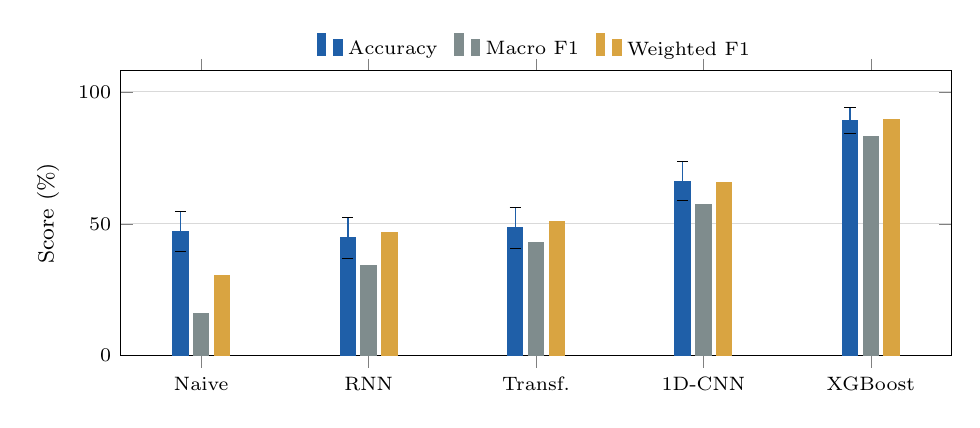
\begin{tikzpicture}
\begin{axis}[ybar,width=\columnwidth,height=5.2cm,bar width=5.5pt,
  symbolic x coords={Naive,RNN,Transf.,1D-CNN,XGBoost},xtick=data,
  ymin=0,ymax=108,ylabel={Score (\%)},
  tick label style={font=\scriptsize},label style={font=\footnotesize},
  ymajorgrids,grid style={gray!30,thin},
  enlarge x limits=0.12,
  legend columns=3,legend style={font=\scriptsize,draw=none,fill=none,at={(0.5,1.0)},anchor=south,/tikz/every even column/.append style={column sep=4pt}}]
\addplot[fill=bsblue,draw=bsblue,error bars/.cd,y dir=both,y explicit,error bar style={line width=0.5pt}]
  coordinates{(Naive,47.1) +- (0,7.7) (RNN,44.6) +- (0,7.7) (Transf.,48.4) +- (0,7.75) (1D-CNN,66.2) +- (0,7.35) (XGBoost,89.2) +- (0,4.9)};
\addplot[fill=bsgray,draw=bsgray]coordinates{(Naive,16.0) (RNN,34.0) (Transf.,42.9) (1D-CNN,57.2) (XGBoost,83.2)};
\addplot[fill=bsgold,draw=bsgold]coordinates{(Naive,30.2) (RNN,46.8) (Transf.,50.8) (1D-CNN,65.7) (XGBoost,89.4)};
\legend{Accuracy,Macro F1,Weighted F1}
\end{axis}
\end{tikzpicture}
\caption{Accuracy, macro F1 and weighted F1 of the five models on the held-out test set. Whiskers show the 95\% Wilson interval of accuracy.}
\label{fig:models}
\end{figure}

Table V and Fig.~\ref{fig:perclass} give the per-class results. XGBoost reaches F1 scores of 72.0, 91.3, 91.8 and 77.8\% for LOW, MEDIUM, HIGH and CRITICAL. The minority tiers are the weakest: LOW precision is 64.3\% (9 of 14 predictions), and CRITICAL recall is 7 of 9. With only nine test records, the 77.8\% CRITICAL recall has a 95\% Wilson interval of 45.3--93.7\% and should not be over-interpreted.

\begin{table}[!t]
\centering
\tcap{V}{XGBoost Per-Class Test Metrics}
\footnotesize
\begin{tabular}{|l|c|c|c|c|}
\hline
\textbf{Tier} & \textbf{Precision} & \textbf{Recall} & \textbf{F1} & \textbf{Support}\\
\hline
LOW & 64.3 & 81.8 & 72.0 & 11\\
\hline
MEDIUM & 90.7 & 91.9 & 91.3 & 74\\
\hline
HIGH & 94.9 & 88.9 & 91.8 & 63\\
\hline
CRITICAL & 77.8 & 77.8 & 77.8 & 9\\
\hline
\end{tabular}
\tnote{Scores are in percent.}
\end{table}

\begin{figure}[!t]
\centering
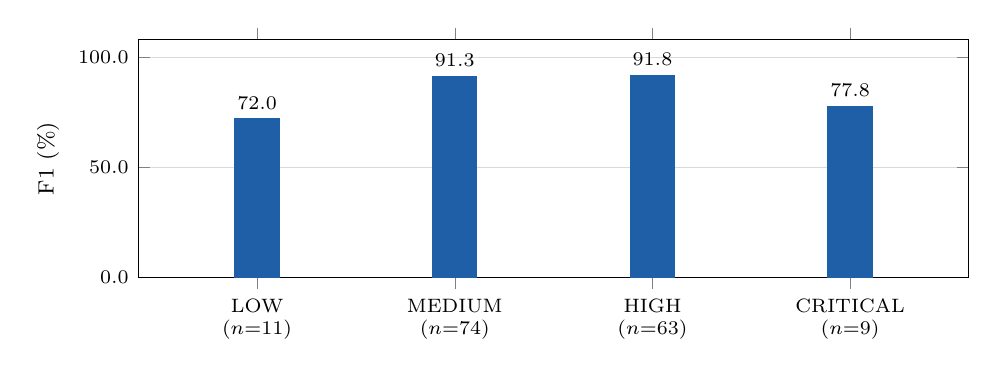
\begin{tikzpicture}
\begin{axis}[ybar,width=\columnwidth,height=4.6cm,bar width=16pt,
  xtick={0,1,2,3},xticklabels={LOW\\($n{=}11$),MEDIUM\\($n{=}74$),HIGH\\($n{=}63$),CRITICAL\\($n{=}9$)},
  xticklabel style={align=center},
  xmin=-0.6,xmax=3.6,ymin=0,ymax=108,ylabel={F1 (\%)},
  tick label style={font=\scriptsize},label style={font=\footnotesize},
  ymajorgrids,grid style={gray!30,thin},
  nodes near coords,nodes near coords align={vertical},
  every node near coord/.append style={font=\scriptsize},
  /pgf/number format/.cd,fixed,fixed zerofill,precision=1]
\addplot[fill=bsblue,draw=bsblue]coordinates{(0,72.0) (1,91.3) (2,91.8) (3,77.8)};
\end{axis}
\end{tikzpicture}
\caption{Per-class F1 of XGBoost. Here $n$ is the test support of each tier.}
\label{fig:perclass}
\end{figure}

XGBoost misclassifies 17 of the 157 test records. Table VI gives the false-positive and false-negative counts for each tier. We derived them from the per-class precision, recall and support in Table V, so the full confusion matrix is not reproduced here. The largest single source of error is the HIGH tier, where 7 of the 63 records are assigned to another tier, while MEDIUM absorbs 7 false positives. LOW has the lowest precision, with 5 false positives against 9 correct predictions, which is unsurprising for a tier with only 11 test records. In our evaluation the errors fell mostly on adjacent tiers, for example MEDIUM predicted as HIGH, which is the less costly failure mode for a triage system.

\begin{table}[!t]
\centering
\tcap{VI}{XGBoost Error Counts on the Test Set}
\footnotesize
\begin{tabular}{|l|c|c|c|c|c|}
\hline
\textbf{Tier} & \textbf{Support} & \textbf{Predicted} & \textbf{Correct} & \textbf{FP} & \textbf{FN}\\
\hline
LOW & 11 & 14 & 9 & 5 & 2\\
\hline
MEDIUM & 74 & 75 & 68 & 7 & 6\\
\hline
HIGH & 63 & 59 & 56 & 3 & 7\\
\hline
CRITICAL & 9 & 9 & 7 & 2 & 2\\
\hline
\textbf{All} & \textbf{157} & \textbf{157} & \textbf{140} & \textbf{17} & \textbf{17}\\
\hline
\end{tabular}
\tnote{FP: false positives; FN: false negatives. Derived from per-class precision, recall and support.}
\end{table}

\subsection{Analysis and Deployment Status}

The margin is consistent with the finding that tree ensembles remain strong on medium-sized tabular data [20]. We have not isolated the cause experimentally, but a plausible explanation is that the DataClasses vocabulary is an unordered, sparse categorical space. Recurrent and attention architectures impose sequence or position structure on such a space, whereas axis-aligned splits do not.

XGBoost is not the production scorer. The search path uses the deterministic function of Section IV-D, because live OSINT feeds do not reliably supply all the fields that the classifier's feature contract requires (DataClasses, volume and verification flag). The UrlBERT classifier does run on the search path, and a known phishing URL returned a phishing confidence of 0.9999. This is a functional check on a single instance, not an accuracy evaluation.

\subsection{Summary of Findings}

\textbf{RQ1.} A range request discloses at most 20 bits of the target digest \eqref{eq:leak}. With $N=1{,}034$ the expected bucket size is $9.9\times10^{-4}$ \eqref{eq:bucket}, so the present anonymity set is effectively one, and the authentication channel can disclose the queried identifier to the operator. The guarantee is therefore conditional on corpus growth and on separating the authenticating identity from the searched identifier.

\textbf{RQ2.} The Merkle construction was verified and the contract compiles. Unanchored events are exposed for at most $T_{\max}$ plus the confirmation time \eqref{eq:window}, provided the anchoring node confirms the transaction. Deployment currently fails because the deployer credential is not set, so we do not claim end-to-end anchoring.

\textbf{RQ3.} XGBoost reaches 89.2\% accuracy (95\% CI 83.3--93.1) against 66.2\% (58.5--73.2) for the 1D-CNN, and the intervals do not overlap. The Transformer and the recurrent network are statistically indistinguishable from the naive baseline. CRITICAL recall is 7 of 9, with a wide interval.

% =====================  VII. VERIFICATION  =====================
\section{Verification of the Implementation}

\subsection{Method}

A substantial part of the code base was produced with AI coding assistants, so we kept a result only if we could confirm it by running the system or reading its source. We ran two independently prompted audits of the code base, and neither had access to the other's output. Where they disagreed, we settled the question with live commands against the running system instead of choosing between the two reports. A third party then re-derived the reported results from raw data and source in an isolated environment. This process removed claims that could not be reproduced, including performance figures that had no underlying measurement, which is why we report no system-level latency benchmark.

\subsection{Outcome}

Table VII summarises the outcome. Two items did not pass. First, the anchoring deployment script fails in the evaluation environment because the deployer credential is not set. The signer list is empty, so the script cannot read a deployer address. This is a configuration defect rather than a flaw in the batching logic, but it means we cannot claim end-to-end anchoring as verified. Second, two of the four source adapters do not yet perform outbound calls.

\begin{table}[!t]
\centering
\tcap{VII}{Verification Summary}
\footnotesize
\setlength{\tabcolsep}{3pt}
\begin{tabular}{|p{0.22\columnwidth}|p{0.34\columnwidth}|p{0.34\columnwidth}|}
\hline
\textbf{Component} & \textbf{Method} & \textbf{Outcome}\\
\hline
Range search & Live HTTP requests; source inspection & Correct prefix and bucket round trip\\
\hline
Severity classifier & Repeated inference; independent instantiation & Identical outputs; checkpoint loaded\\
\hline
URL classifier & Known phishing URL & Functioning; confidence 0.9999\\
\hline
Exposure scoring & Live requests; source inspection & Computed from record data, not constants\\
\hline
Backend tests & Automated suite & 101/101 pass (26 suites), also with OTP enforced\\
\hline
Frontend tests & Automated suite & 50/50 pass (3 suites)\\
\hline
Merkle batching & Construction check; contract compile & Construction verified; contract compiles\\
\hline
Anchor deployment & Clean local deployment & Fails: deployer credential unset\\
\hline
Source adapters & Source inspection & 2 of 4 perform outbound calls\\
\hline
\end{tabular}
\end{table}

% =====================  VIII. LIMITATIONS  =====================
\section{Limitations and Threats to Validity}

\begin{enumerate}[label=\Alph*.,leftmargin=1.6em,itemsep=2pt]
\item \textit{Anonymity set.} At $N=1{,}034$ the expected bucket holds only about $10^{-3}$ entries (Section V-B), so privacy rests on the 20-bit prefix bound alone.
\item \textit{Authentication linkage.} Because the session token carries the target identifier, the operator can learn it through the authentication channel (Section V-A).
\item \textit{Dataset.} The benchmark uses 1,034 records, one stratified split and just nine CRITICAL test records. The procedure that assigned the severity labels determines what the benchmark actually measures. If the labels are a function of the DataClasses features, high accuracy from a tree ensemble is expected and does not show that the model generalises to independently labelled breaches. We did not evaluate on external data, and we did not apply resampling such as SMOTE [9].
\item \textit{Production path.} The classifier is not on the search path. The deployed scorer is explainable, but we have not evaluated it against labelled outcomes.
\item \textit{Anchoring.} Anchoring currently targets a local EVM node, and deployment fails until a deployer credential is supplied, so we make no claim of public verifiability. Events that have not yet been anchored stay exposed for up to $T_{\max}$ plus the confirmation time.
\item \textit{Coverage.} Two of the four adapters are still placeholders, and the only live external feed is the Telegram-channel scraper.
\item \textit{Operations.} A development-only OTP bypass flag exists and must be switched off in any real deployment. The bcrypt and OTP parameters follow common practice, but we did not load-test them against adversarial request volumes. In the calls we observed, UrlBERT inference took roughly 14--31\,ms per request, which should be read as an observation and not as an aggregate or percentile latency figure.
\end{enumerate}

% =====================  IX. CONCLUSION  =====================
\section{Conclusion and Future Work}

BreachShield combines a client-side k-anonymous range query, an OTP-gated session, a bounded and explainable exposure score and a Merkle-batched audit log. In this paper we examined what each component does and does not guarantee. The range query limits payload leakage to 20 bits, but at the present corpus size the anonymity set is effectively one, and the authentication channel can still expose the queried identifier. Batching leaves an exposure window that we can state exactly: at most $T_{\max}$ plus the confirmation time. On 1,034 records XGBoost outperforms the neural baselines, although the estimate for the rarest class remains uncertain.

Our future work, in priority order, is as follows. First, we will supply the deployer credential and verify anchoring end to end. Second, we will decouple the authenticating identity from the queried identifier, or adopt private-set-intersection protocols [4]. Third, we will grow the corpus or pad the buckets so that the anonymity set becomes meaningful. Fourth, we will evaluate the classifier on independently labelled data and resample the CRITICAL tier [9]. Fifth, we will implement the remaining source adapters and run a reproducible latency benchmark before making any performance claim. Anchoring to a public chain, using a batching design such as the one in [18], is a longer-term option once local verification is complete.

\section*{Acknowledgment}

This work was carried out as part of Project Phase II (BIS786) at the Department of Information Science and Engineering, Acharya Institute of Technology, Bengaluru, India.

% =====================  REFERENCES  =====================
\begingroup
\section*{References}
\fontsize{8}{9.4}\selectfont
\setlength{\parindent}{0pt}
\newcounter{refctr}
\newcommand{\bref}[1]{\stepcounter{refctr}\par\hangindent=2.1em\hangafter=1\noindent\makebox[2.1em][l]{[\arabic{refctr}]}#1\par\vspace{1.5pt}}

\bref{IBM Security, ``Cost of a data breach report 2024,'' IBM Corporation, Jul. 2024.}
\bref{K. Thomas \textit{et al.}, ``Protecting accounts from credential stuffing with password breach alerting,'' in \textit{Proc. 28th USENIX Security Symp.}, 2019, pp. 1556--1571.}
\bref{J. Ali, ``Validating leaked passwords with k-anonymity,'' Cloudflare Blog, Feb. 21, 2018. [Online]. Available: \url{https://blog.cloudflare.com/validating-leaked-passwords-with-k-anonymity/}}
\bref{L. Li, B. Pal, J. Ali, N. Sullivan, R. Chatterjee, and T. Ristenpart, ``Protocols for checking compromised credentials,'' in \textit{Proc. ACM SIGSAC Conf. Comput. Commun. Secur. (CCS)}, 2019, pp. 1387--1403.}
\bref{L. Sweeney, ``k-Anonymity: A model for protecting privacy,'' \textit{Int. J. Uncertainty, Fuzziness Knowl.-Based Syst.}, vol. 10, no. 5, pp. 557--570, 2002.}
\bref{K. El Emam and F. K. Dankar, ``Protecting privacy using k-anonymity,'' \textit{J. Amer. Med. Inform. Assoc.}, vol. 15, no. 5, pp. 627--637, 2008.}
\bref{A. Aljofey, Q. Jiang, Q. Qu, M. Huang, and J.-P. Niyigena, ``An effective phishing detection model based on character level convolutional neural network from URL,'' \textit{Electronics}, vol. 9, no. 9, Art. no. 1514, 2020.}
\bref{O. K. Sahingoz, E. Buber, and E. Kugu, ``DEPHIDES: Deep learning based phishing detection system,'' \textit{IEEE Access}, vol. 12, pp. 8052--8070, 2024, doi: 10.1109/ACCESS.2024.3352629.}
\bref{F. S. Alsubaei, A. A. Almazroi, and N. Ayub, ``Enhancing phishing detection: A novel hybrid deep learning framework for cybercrime forensics,'' \textit{IEEE Access}, vol. 12, 2024.}
\bref{B. V. Pavani, D. Mahitha, and B. Uma Maheswari, ``Enhancing online safety: Phishing URL detection using machine learning and explainable AI,'' in \textit{Proc. 15th Int. Conf. Comput. Commun. Netw. Technol. (ICCCNT)}, 2024, pp. 1--6, doi: 10.1109/ICCCNT61001.2024.10723976.}
\bref{M. Tawfik, A. A. Abu-Ein, A. H. Abdelhaliem, Y. M. Al-Sharo, and I. S. Fathi, ``Explainable few-shot learning with modern BERT for detecting emerging phishing attacks using XF-PhishBERT,'' \textit{Sci. Rep.}, vol. 15, Art. no. 42821, 2025, doi: 10.1038/s41598-025-27500-0.}
\bref{P. K\"uhn, K. Wittorf, and C. Reuter, ``Navigating the shadows: Manual and semi-automated evaluation of the dark web for cyber threat intelligence,'' \textit{IEEE Access}, vol. 12, pp. 118903--118922, 2024, doi: 10.1109/ACCESS.2024.3448247.}
\bref{M. Saleem, R. Islam, and M. A. Kabir, ``The anonymity of the dark web: A survey,'' \textit{IEEE Access}, vol. 10, 2022.}
\bref{J. Pastor-Galindo, P. Nespoli, F. G\'omez M\'armol, and G. Mart\'inez P\'erez, ``The not yet exploited goldmine of OSINT: Opportunities, open challenges and future trends,'' \textit{IEEE Access}, vol. 8, pp. 10282--10304, 2020, doi: 10.1109/ACCESS.2020.2965257.}
\bref{R. C. Merkle, ``A digital signature based on a conventional encryption function,'' in \textit{Advances in Cryptology---CRYPTO '87}. Berlin, Germany: Springer, 1988, pp. 369--378.}
\bref{S. A. Crosby and D. S. Wallach, ``Efficient data structures for tamper-evident logging,'' in \textit{Proc. 18th USENIX Security Symp.}, 2009.}
\bref{B. Laurie, A. Langley, and E. Kasper, ``Certificate Transparency,'' IETF, RFC 6962, Jun. 2013.}
\bref{A. Arabnouri, S. Eissazadeh, and A. Shafieinejad, ``A secure auditable log based on blockchain,'' \textit{Monadi}, vol. 13, no. 2, pp. 75--86, 2024.}
\bref{T. Chen and C. Guestrin, ``XGBoost: A scalable tree boosting system,'' in \textit{Proc. 22nd ACM SIGKDD Int. Conf. Knowl. Discovery Data Mining}, 2016, pp. 785--794.}
\bref{L. Grinsztajn, E. Oyallon, and G. Varoquaux, ``Why do tree-based models still outperform deep learning on typical tabular data?'' in \textit{Proc. Adv. Neural Inf. Process. Syst. (NeurIPS)}, 2022.}
\bref{M. Jones, J. Bradley, and N. Sakimura, ``JSON Web Token (JWT),'' IETF, RFC 7519, May 2015.}
\bref{N. Provos and D. Mazi\`eres, ``A future-adaptable password scheme,'' in \textit{Proc. USENIX Annu. Tech. Conf., FREENIX Track}, 1999, pp. 81--91.}
\endgroup

\end{document}
